Tidyparse offers a user interface featuring a text editor, a grammar editor and a parse tree viewer for interactive prototyping. For example, suppose we have the following context-free grammar:

\begin{wholetidyinput}
S -> S and S | S xor S | ( S ) | true | false | ! S(*@\caret{ }@*)
\end{wholetidyinput}

\noindent As described in Sec.~\ref{sec:matrix}, this is automatically be rewritten into the grammar:

\begin{verbatim}
 F.! → !     S.) → S F.)  and.S → F.and S   S → F.! S     S → false    S → S ε+
 F.( → (   F.xor → xor    xor.S → F.xor S   S → S and.S   S → true    ε+ → ε
 F.) → )   F.and → and        S → S xor.S   S → F.( S.)   S → <S>     ε+ → ε+ ε+
\end{verbatim}

%\noindent We can visualize the CFG as either a graph or a matrix:
%
%\begin{figure}[H]
%    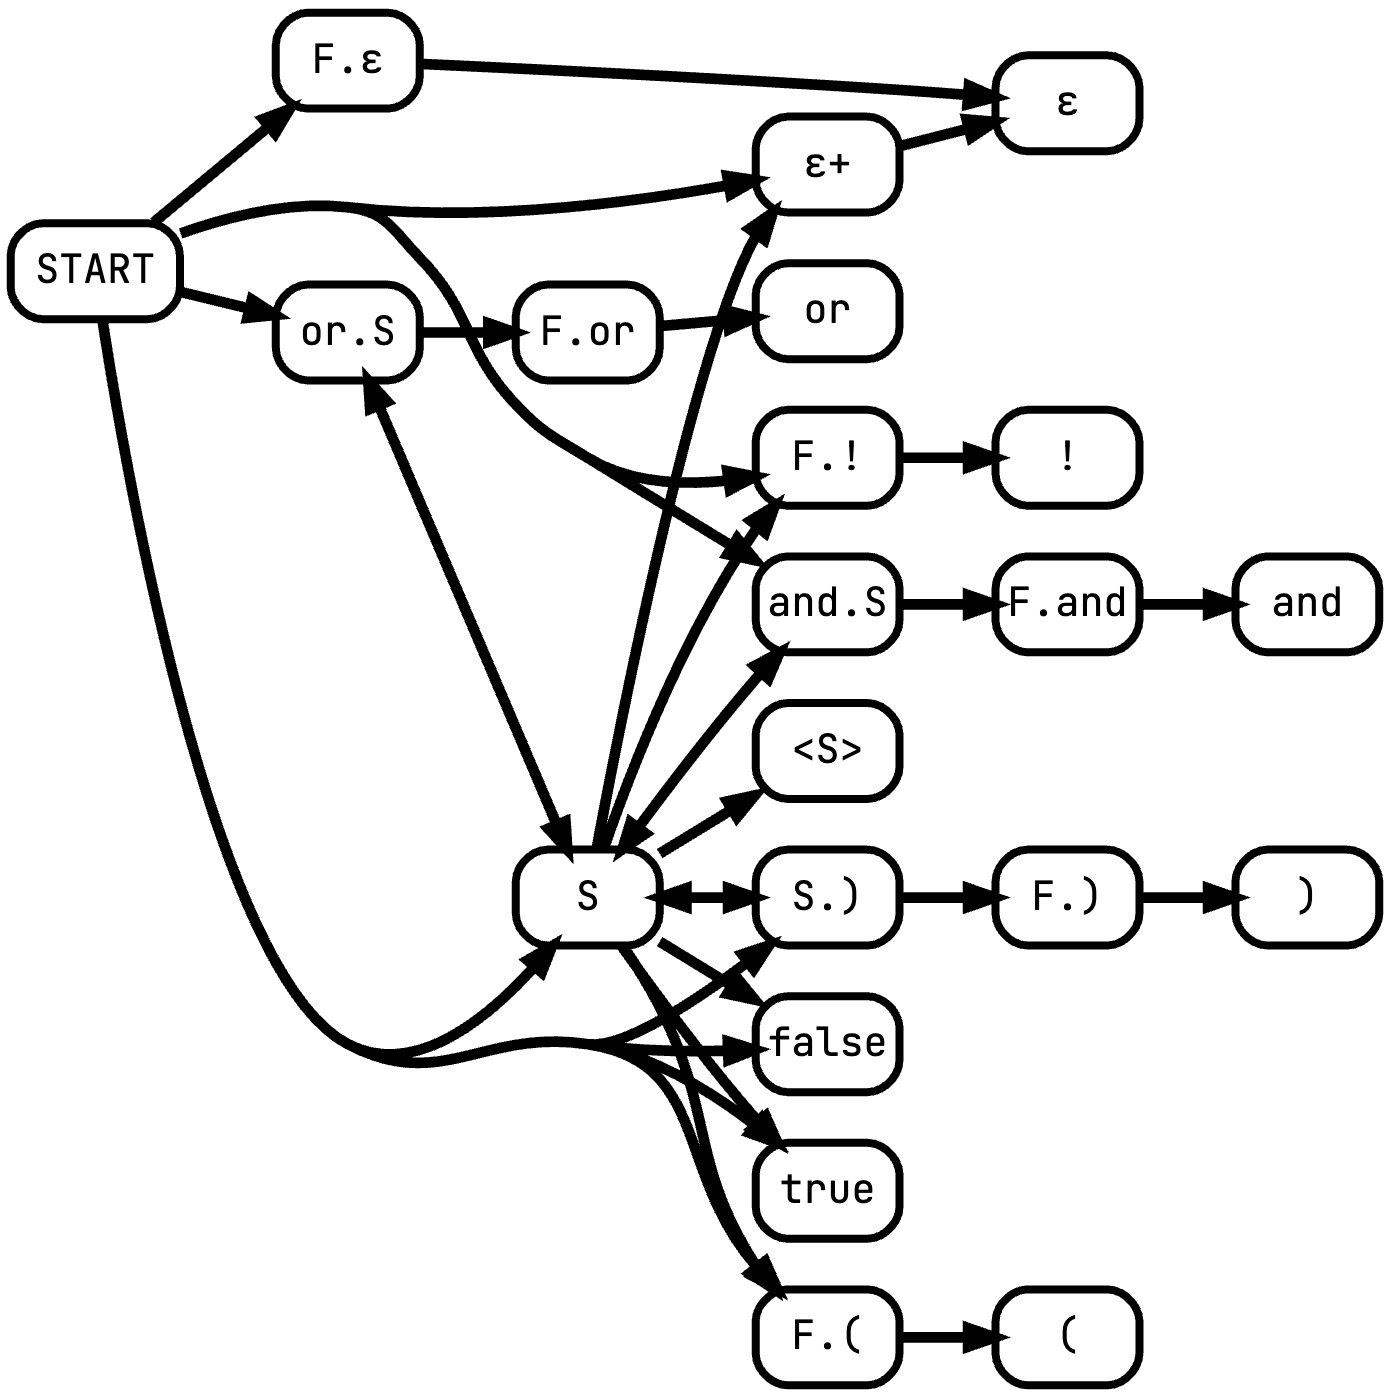
\includegraphics[width=3.5cm]{../figures/bool_arith_cfg_graph.png}
%    \hspace{20pt}
%    \includegraphics[width=3.5cm]{../figures/bool_arith_cfg_mat.bmp}
%\end{figure}

\noindent Given a string containing holes, our tool will return several completions in a few milliseconds:

\begin{tcolorbox}[left skip=0.7cm,
top=0.1cm,
middle=0mm,
boxsep=0mm,
underlay unbroken and first={%
    \path[draw=none] (interior.north west) rectangle node[white]{
\includegraphics[width=4mm]{../figures/tidyparse_logo.png}} ([xshift=-10mm,yshift=-9mm]interior.north west);
}]
  \begin{lstlisting} [language=tidy, basicstyle=\ttfamily\small, escapeinside={(*@}{@*)}]
true _ _ _ ( false _ ( _ _ _ _ ! _ _ ) _ _ _ _(*@\caret{ }@*)
  \end{lstlisting}
  \tcblower
  \begin{lstlisting} [language=tidy, basicstyle=\ttfamily\small, escapeinside={(*@}{@*)}]
1. true (*@\hlorange{xor}@*) (*@\hlorange{!}@*) ( false (*@\hlorange{xor}@*) ( (*@\hlorange{<S>}@*) (*@\hlorange{)}@*) (*@\hlorange{or}@*) ! (*@\hlorange{<S>}@*) ) (*@\hlorange{xor}@*) (*@\hlorange{<S>}@*)
2. true (*@\hlorange{xor}@*) (*@\hlorange{!}@*) ( false (*@\hlorange{and}@*) ( (*@\hlorange{<S>}@*) (*@\hlorange{)}@*) (*@\hlorange{or}@*) ! (*@\hlorange{<S>}@*) ) (*@\hlorange{xor}@*) (*@\hlorange{<S>}@*)
3. true (*@\hlorange{xor}@*) (*@\hlorange{!}@*) ( false (*@\hlorange{and}@*) ( (*@\hlorange{<S>}@*) (*@\hlorange{)}@*) (*@\hlorange{and}@*) ! (*@\hlorange{<S>}@*) ) (*@\hlorange{xor}@*) (*@\hlorange{<S>}@*)
4. true (*@\hlorange{xor}@*) (*@\hlorange{!}@*) ( false (*@\hlorange{and}@*) ( (*@\hlorange{<S>}@*) (*@\hlorange{)}@*) (*@\hlorange{and}@*) ! (*@\hlorange{<S>}@*) ) (*@\hlorange{and}@*) (*@\hlorange{<S>}@*)
...
  \end{lstlisting}
\end{tcolorbox}

\noindent Similarly, if provided with a string containing various errors, it will return several suggestions how to fix it, where \hlgreen{green} is insertion, \hlorange{orange} is substitution and \hlred{red} is deletion.

\begin{tcolorbox}[left skip=0.7cm,
top=0.1cm,
middle=0mm,
boxsep=0mm,
underlay unbroken and first={%
    \path[draw=none] (interior.north west) rectangle node[white]{
\includegraphics[width=4mm]{../figures/tidyparse_logo.png}} ([xshift=-10mm,yshift=-9mm]interior.north west);
}]
\begin{lstlisting} [language=tidy, basicstyle=\ttfamily\small, escapeinside={(*@}{@*)}]
true and ( false or and true false(*@\caret{ }@*)
\end{lstlisting}
\tcblower
\begin{lstlisting} [language=tidy, basicstyle=\ttfamily\small, escapeinside={(*@}{@*)}]
1. true and ( false or (*@\hlorange{!}@*) true (*@\hlorange{)}@*)
2. true and ( false or (*@\hlgreen{<S>}@*) and true (*@\hlorange{)}@*)
3. true and ( false or (*@\hlorange{(}@*) true (*@\hlorange{)}@*) (*@\hlgreen{)}@*)
...
9. true and ( false or (*@\hlgreen{!}@*) (*@\hlgreen{<S>}@*) (*@\hlgreen{)}@*) and true (*@\hlred{false} @*)
\end{lstlisting}
\end{tcolorbox}

Since CFLs are closed under homomorphisms, it is possible to unify lexing and parsing, however most languages explicitly define a separate lexer, which we avail to substitute named identifiers with their type. Given an invalid string, the tool will first abstract the raw characters, generate edits in the abstract token space, then remap successful repairs back to character space as shown below:

\hspace{-0.4cm}\begin{minipage}[t]{0.485\textwidth}
\begin{tcolorbox}[
left skip=0.7cm,
left=0.35cm,
right=0cm,
top=0.1cm,
middle=0mm,
boxsep=0mm,
underlay unbroken and first={%
  \path[draw=none] (interior.north west) rectangle node[white]{
\includegraphics[width=4mm]{../figures/tidyparse_logo.png}} ([xshift=-10mm,yshift=-9mm]interior.north west);
}]
\begin{lstlisting} [hbox, language=tidy, basicstyle=\ttfamily\small, escapeinside={(*@}{@*)}]
d = sum([foo(i] for i in vals))(*@\caret{ }@*)
\end{lstlisting}
\tcblower
\begin{lstlisting} [hbox, language=tidy, basicstyle=\ttfamily\small, escapeinside={(*@}{@*)}]
1. d = sum([foo(i(*@\hlorange{)}@*) for i in vals(*@\hlorange{]}@*))
2. d = sum([(i(*@\hlorange{)}@*) for i in vals(*@\hlorange{]}@*))
3. d = sum([foo(*@\hlorange{.}@*)i for i in vals(*@\hlorange{]}@*))
4. d = sum([foo((*@\hlgreen{+}@*)i(*@\hlorange{)}@*) for i in vals(*@\hlorange{]}@*))
\end{lstlisting}
\end{tcolorbox}
\end{minipage}
\hspace{0.05cm}
\begin{minipage}[t]{0.51\textwidth}
\begin{tcolorbox}[
left skip=0.7cm,
left=0.35cm,
right=0cm,
top=0.1cm,
middle=0mm,
boxsep=0mm,
underlay unbroken and first={%
  \path[draw=none] (interior.north west) rectangle node[white]{
\includegraphics[width=4mm]{../figures/tidyparse_logo.png}} ([xshift=-10mm,yshift=-9mm]interior.north west);
}]
\begin{lstlisting} [language=tidy, basicstyle=\ttfamily\small, escapeinside={(*@}{@*)}]
w = w ( [ w ( w ] for w in w ) )
\end{lstlisting}
\tcblower
\begin{lstlisting} [language=tidy, basicstyle=\ttfamily\small, escapeinside={(*@}{@*)}]
1. w = w ( [ w ( i (*@\hlorange{)}@*) for i in w (*@\hlorange{]}@*) )
2. w = w ( [ (*@\hlred{w}@*) ( w (*@\hlorange{)}@*) for w in w (*@\hlorange{]}@*) )
3. w = w ( [ w (*@\hlorange{.}@*) w (*@\hlred{)}@*)  for w in w (*@\hlorange{]}@*) )
4. w = w ( [ w ( (*@\hlgreen{+}@*) w (*@\hlorange{)}@*) for w in w (*@\hlorange{)}@*) )
\end{lstlisting}
\end{tcolorbox}
\end{minipage}

This coarsening reduces the number of possible corrections, although is not strictly necessary. For simplicity, it is also possible to define a grammar and string side-by-side, as shown in the untyped \lambda-calculus example below:

\begin{tcolorbox}[left skip=0.7cm,
top=0.1cm,
middle=0mm,
boxsep=0mm,
underlay unbroken and first={%
  \path[draw=none] (interior.north west) rectangle node[white]{
\includegraphics[width=4mm]{../figures/tidyparse_logo.png}} ([xshift=-10mm,yshift=-9mm]interior.north west);
}]
\begin{lstlisting} [language=tidy, basicstyle=\ttfamily\small, escapeinside={(*@}{@*)}]
sxp -> λ var . sxp | sxp sxp | var | ( sxp )
var -> a | b | c | f | x | y | z
---
( λ f . ( λ x . f ( x x ) ) ( λ x . f ( x x ) (*@\caret{ }@*)
\end{lstlisting}
\tcblower
\begin{lstlisting} [language=tidy, basicstyle=\ttfamily\small, escapeinside={(*@}{@*)}]
1. ( λ f . ( λ x . f ( x x ) ) (*@\hlorange{)}@*) λ x . f ( x x )
2. ( λ f . ( λ x . f ( x x ) ) (*@\hlorange{x}@*) (*@\hlgreen{)}@*) λ x . f ( x x )
3. ( λ f . ( λ x . f ( x x ) ) ( λ x . f ( x(*@\hlred{ }@*)) (*@\hlgreen{)}@*) (*@\hlgreen{)}@*)
\end{lstlisting}
\end{tcolorbox}

\noindent Name resolution and scope checking is also possible but requires a more sophisticated grammar.

\subsection{Syntax highlighting}

We use the parse forest from \S\ref{sec:error_recovery} to segment maximally parseable regions. Subsequences which can be partly parsed are underlined in blue. Alphabetic tokens which cannot be joined are marked orange. All other tokens are marked red.

\begin{tcolorbox}[left skip=0.7cm,
top=0.1cm,
middle=0mm,
boxsep=0mm,
underlay unbroken and first={%
  \path[draw=none] (interior.north west) rectangle node[white]{
\includegraphics[width=4mm]{../figures/tidyparse_logo.png}} ([xshift=-10mm,yshift=-9mm]interior.north west);
}]
\begin{lstlisting} [language=tidy, basicstyle=\ttfamily\small, escapeinside={(*@}{@*)}]
(*@\erb{( true xor false ) and true}@*) (*@\ero{xor}@*)  (*@\ero{and}@*)  (*@\err{not}@*) (*@\ero{false}@*)
\end{lstlisting}
\end{tcolorbox}

\subsection{Grammar assistance}

Tidyparse uses a CFG to parse the CFG, so it can provide editing assistance while the user is designing the CFG. For example, if the CFG does not parse, will suggest a list of possible fixes.% In the future, we intend to use this functionality to perform example-based codesign and grammar induction.

\hspace{-0.4cm}\begin{minipage}[t]{0.485\textwidth}
\begin{tcolorbox}[
left skip=0.7cm,
left=0.35cm,
right=0cm,
top=0.1cm,
middle=0mm,
boxsep=0mm,
underlay unbroken and first={%
 \path[draw=none] (interior.north west) rectangle node[white]{
\includegraphics[width=4mm]{../figures/tidyparse_logo.png}} ([xshift=-10mm,yshift=-9mm]interior.north west);
}]
\begin{lstlisting} [hbox, language=tidy, basicstyle=\ttfamily\small, escapeinside={(*@}{@*)}]
START -> CFG
CFG -> PRD | CFG \n CFG
PRD -> TOK '->' RHS
TOK -> [A-Za-z']+
RHS -> TOK | RHS RHS | RHS '|' RHS
\end{lstlisting}
\end{tcolorbox}
\end{minipage}
\hspace{0.05cm}
\begin{minipage}[t]{0.51\textwidth}
  \begin{tcolorbox}[
  left skip=0.7cm,
  left=0.35cm,
  right=0cm,
  top=0.1cm,
  middle=0mm,
  boxsep=0mm,
  underlay unbroken and first={%
    \path[draw=none] (interior.north west) rectangle node[white]{
\includegraphics[width=4mm]{../figures/tidyparse_logo.png}} ([xshift=-10mm,yshift=-9mm]interior.north west);
  }]
  \begin{lstlisting} [language=tidy, basicstyle=\ttfamily\small, escapeinside={(*@}{@*)}]
B ::= true | false | (*@\caret{ }@*)
  \end{lstlisting}
  \tcblower
  \begin{lstlisting} [language=tidy, basicstyle=\ttfamily\small, escapeinside={(*@}{@*)}]
1. B (*@\hlorange{->}@*) true | false (*@\hlred{ }@*)
2. B (*@\hlorange{->}@*) true | false (*@\hlorange{<RHS>}@*)
3. B (*@\hlorange{->}@*) true | false | (*@\hlgreen{<RHS>}@*)
  \end{lstlisting}
  \end{tcolorbox}
\end{minipage}

\subsection{Interactive nonterminal expansion}

Users can interactively build up a complex expression by placing the caret over a nonterminal they wish to expand, then pressing \keys{\ctrl + \SPACE} to receive a list of possible substitutions.

\begin{tcolorbox}[left skip=0.7cm,
top=0.1cm,
middle=0mm,
boxsep=0mm,
underlay unbroken and first={%
  \path[draw=none] (interior.north west) rectangle node[white]{
\includegraphics[width=4mm]{../figures/tidyparse_logo.png}} ([xshift=-10mm,yshift=-9mm]interior.north west);
}]
\begin{lstlisting} [language=tidy, basicstyle=\ttfamily\small, escapeinside={(*@}{@*)}]
true and ( false or <(*@\caret{S}@*)> and true )
\end{lstlisting}
\tcblower
\begin{lstlisting} [language=tidy, basicstyle=\ttfamily\small, escapeinside={(*@}{@*)}]
1. true and ( false or (*@\hlorange{true}@*) and true )
2. true and ( false or (*@\hlorange{false}@*) and true )
3. true and ( false or (*@\hlorange{! <S>}@*) and true )
\end{lstlisting}
\end{tcolorbox}

\subsection{Nonterminal stubs}

Tidyparse augments CFGs with two additional rules, which are desugared into a vanilla CFG before parsing. The first rule, $\alpha\textsc{-sub}$, allows the user to define a nonterminal parameterized by $\alpha$, a non-recursive nonterminal in the same the CFG representing some finite type and its inhabitants. $\alpha\textsc{-sub}$ replaces all productions containing $\langle\alpha\rangle$ with the terminals in their transitive closure, $\alpha \rightarrow^* \beta$. The second rule, $\alpha\textsc{-int}$, introduces homonymous terminals for each user-defined nonterminal.

\begin{figure}[H]
  \begin{prooftree}
    \AxiomC{$\mathcal{G} \vdash (w\langle\alpha\rangle \rightarrow x z) \in P$}
    \AxiomC{$\alpha^* : \{\beta \mid (\alpha \rightarrow^* \beta) \in P\}$}
    \RightLabel{$\alpha\textsc{-sub}$}
    \BinaryInfC{$\mathcal{G} \vdash \forall \beta \in \alpha^*.(w\langle\alpha\rangle \rightarrow x z)[\beta/\alpha] \in P'$}
    \DisplayProof
    \hskip 1.5em
    \AxiomC{$\mathcal{G} \vdash v \in V$}
    \RightLabel{$\langle\cdot\rangle\textsc{-int}$}
    \UnaryInfC{$\mathcal{G} \vdash (v \rightarrow \langle v\rangle) \in P$}
  \end{prooftree}
\end{figure}

Tidyparse can also perform a limited form of type checking. Typed expressions are automatically expanded into ordinary nonterminals using the $\alpha\textsc{-sub}$ rule, for example when parsing an expression of the form $x + y$, the grammar will recognize \texttt{true + false} and \texttt{1 + 2}, but not \texttt{1 + true}.

\begin{tcolorbox}[left skip=0.7cm,
top=0.1cm,
middle=0mm,
boxsep=0mm,
underlay unbroken and first={%
  \path[draw=none] (interior.north west) rectangle node[white]{
\includegraphics[width=4mm]{../figures/tidyparse_logo.png}} ([xshift=-10mm,yshift=-9mm]interior.north west);
}]
\begin{lstlisting} [language=tidy, basicstyle=\ttfamily\small, escapeinside={(*@}{@*)}]
E<X> -> E<X> + E<X> | E<X> * E<X> | ( E<X> )
X -> Int | Bool
\end{lstlisting}
\tcblower
\begin{lstlisting} [language=tidy, basicstyle=\ttfamily\small, escapeinside={(*@}{@*)}]
E<Int> -> E<Int> + E<Int> | E<Int> * E<Int>
E<Bool> -> E<Bool> + E<Bool> | E<Bool> * E<Bool>
\end{lstlisting}
\end{tcolorbox}

\subsection{Conjunctive grammars}

Many natural and programming languages exhibit context-sensitivity, such as Python indentation. Unlike traditional parser-generators, Tidyparse can encode CFL intersection, allowing it to detect and correct errors in a more expressive family of languages than would ordinarily be possible using CFGs alone. For example, consider the grammar from Sec.~\ref{sec:lclreach}:

\hspace{-0.4cm}\begin{minipage}[t]{0.485\textwidth}
\begin{tcolorbox}[
left skip=0.7cm,
left=0.35cm,
right=0cm,
top=0.1cm,
middle=0mm,
boxsep=0mm,
underlay unbroken and first={%
\path[draw=none] (interior.north west) rectangle node[white]{
\includegraphics[width=4mm]{../figures/tidyparse_logo.png}} ([xshift=-10mm,yshift=-9mm]interior.north west);
}]
\begin{lstlisting} [hbox, language=tidy, basicstyle=\ttfamily\small, escapeinside={(*@}{@*)}]
S -> LEFT RIGHT
LEFT -> a b | a LEFT b
RIGHT -> c | c RIGHT
\end{lstlisting}
\end{tcolorbox}
\end{minipage}
\hspace{0.05cm}
\begin{minipage}[t]{0.51\textwidth}
\begin{tcolorbox}[
left skip=0.7cm,
left=0.35cm,
right=0cm,
top=0.1cm,
middle=0mm,
boxsep=0mm,
underlay unbroken and first={%
\path[draw=none] (interior.north west) rectangle node[white]{
\includegraphics[width=4mm]{../figures/tidyparse_logo.png}} ([xshift=-10mm,yshift=-9mm]interior.north west);
}]
\begin{lstlisting} [language=tidy, basicstyle=\ttfamily\small, escapeinside={(*@}{@*)}]
S -> LEFT RIGHT
RIGHT -> b c | b RIGHT c
LEFT -> a | a LEFT
\end{lstlisting}
\end{tcolorbox}
\end{minipage}

\begin{tcolorbox}[left skip=0.7cm,
top=0.1cm,
middle=0mm,
boxsep=0mm,
underlay unbroken and first={%
  \path[draw=none] (interior.north west) rectangle node[white]{
\includegraphics[width=4mm]{../figures/tidyparse_logo.png}} ([xshift=-10mm,yshift=-9mm]interior.north west);
}]
\begin{lstlisting} [language=tidy, basicstyle=\ttfamily\small, escapeinside={(*@}{@*)}]
_ _ _ _ _ _ _ _ _ _ _ _ _ _ _ _ _ _ _ _(*@\caret{ }@*)
\end{lstlisting}
\tcblower
\begin{lstlisting} [language=tidy, basicstyle=\ttfamily\small, escapeinside={(*@}{@*)}]
1. a b c
2. a a b b c c
3. a a a b b b c c c
...
\end{lstlisting}
\end{tcolorbox}

\noindent Tidyparse uses a programmatic interface to signify $\mathcal{L}(\mathcal{G}_1)\cap\mathcal{L}(\mathcal{G}_2)$, i.e., the intersection of two more grammars' languages, as described in \S\ref{sec:lclreach}. This allows the expression of limited indexicality and opens the door to more semantic program analyses like scope checking and name resolution.

%There are some more examples too.
%
%The line between parsing and computation is blurry.
